\documentclass[12pt,letterpaper]{article}
\usepackage{graphicx,textcomp}
\usepackage{natbib}
\usepackage{setspace}
\usepackage{fullpage}
\usepackage{color}
\usepackage[reqno]{amsmath}
\usepackage{amsthm}
\usepackage{fancyvrb}
\usepackage{amssymb,enumerate}
\usepackage[all]{xy}
\usepackage{endnotes}
\usepackage{lscape}
\newtheorem{com}{Comment}
\usepackage{float}
\usepackage{hyperref}
\newtheorem{lem} {Lemma}
\newtheorem{prop}{Proposition}
\newtheorem{thm}{Theorem}
\newtheorem{defn}{Definition}
\newtheorem{cor}{Corollary}
\newtheorem{obs}{Observation}
\usepackage[compact]{titlesec}
\usepackage{dcolumn}
\usepackage{tikz}
\usetikzlibrary{arrows}
\usepackage{multirow}
\usepackage{xcolor}
\newcolumntype{.}{D{.}{.}{-1}}
\newcolumntype{d}[1]{D{.}{.}{#1}}
\definecolor{light-gray}{gray}{0.65}
\usepackage{url}
\usepackage{listings}
\usepackage{color}

\definecolor{codegreen}{rgb}{0,0.6,0}
\definecolor{codegray}{rgb}{0.5,0.5,0.5}
\definecolor{codepurple}{rgb}{0.58,0,0.82}
\definecolor{backcolour}{rgb}{0.95,0.95,0.92}

\lstdefinestyle{mystyle}{
	backgroundcolor=\color{backcolour},   
	commentstyle=\color{codegreen},
	keywordstyle=\color{magenta},
	numberstyle=\tiny\color{codegray},
	stringstyle=\color{codepurple},
	basicstyle=\footnotesize,
	breakatwhitespace=false,         
	breaklines=true,                 
	captionpos=b,                    
	keepspaces=true,                 
	numbers=left,                    
	numbersep=5pt,                  
	showspaces=false,                
	showstringspaces=false,
	showtabs=false,                  
	tabsize=2
}
\lstset{style=mystyle}
\newcommand{\Sref}[1]{Section~\ref{#1}}
\newtheorem{hyp}{Hypothesis}

\title{Problem Set 1}
\date{Due: October 3, 2021}
\author{Applied Stats/Quant Methods 1}

\begin{document}
	\maketitle
	
	\section*{Instructions}
	\begin{itemize}
		\item Please show your work! You may lose points by simply writing in the answer. If the problem requires you to execute commands in \texttt{R}, please include the code you used to get your answers. Please also include the \texttt{.R} file that contains your code. If you are not sure if work needs to be shown for a particular problem, please ask.
		\item Your homework should be submitted electronically on GitHub in \texttt{.pdf} form.
		\item This problem set is due before 8:00 on Friday October 3, 2021. No late assignments will be accepted.
		\item Total available points for this homework is 100.
	\end{itemize}
	
	\vspace{1cm}
	\section*{Question 1 (50 points): Education}
	
	A school counselor was curious about the average of IQ of the students in her school and took a random sample of 25 students' IQ scores. The following is the data set:\\
	\vspace{.5cm}
	
	\vspace{1cm}
	
	\begin{enumerate}
		\item Find a 90\% confidence interval for the average student IQ in the school.\\
		
		Q1.1 Answer:
		
		To find the 90\% Confidence interval for the average student IQ in the school, I first loaded the data set into R Studio by executing the below command. This created an object, y, that was this data set.
		
		\lstinputlisting[language=R, firstline = 52, lastline=52]{PS01.R}	
		
		Next, I calculated the sample mean for this data set with the below command in R Studio:
		
		\lstinputlisting[language=R, firstline=60, lastline=60]{PS01.R}
		
		This produces the value of 98.44, meaning the avg IQ in the sample of 25 students is 98.44. This is the "sample mean".
		
		To check I have calculated the sample mean correctly, I input the following command:
		
		\lstinputlisting[language=R, firstline=67, lastline=67]{PS01.R}
		
		This confirms that my initial calculation of the sample mean is correct.
		
		Next, I calculate the sample's standard deviation, denoted by sd\_y. To do so I must take the square root of the sum of all values in the sample minus the sample mean squared, divided by the sample size minus 1.
		
		I calculate all of these values with the following input into R Studio:
		
		\lstinputlisting[language=R, firstline=76, lastline=82]{PS01.R}
		
		I then calculate the Sample Standard Deviation using the sd() function in R just to confirm my "by hand" calculation was correct:
		
		\lstinputlisting[language=R, firstline=86, lastline=86]{PS01.R}
		
		Both calculations of the sample Standard Deviation produce the outcome of 13.09287, confirming my "by hand" calculation is correct.
		
		Finally, I will use the sample mean and sample standard deviation to calculate the 90\% Confidence Interval (CI) for the avg student IQ in the school.
		CI is the point estimate plus and minus the margin of error.
		Because the Sample Size is small and we are assessing means, we will use a t-distribution to calculate the margin of error.
		The formula I will be putting through R Studio is Mean\_y + and - (t\_0.05)(SE\_y)
		SE\_y is the estimated standard error, which I will calculate first below:
		
		\lstinputlisting[language=R, firstline=99, lastline=99]{PS01.R}
			
		t\_0.05 is 1.711 (according to the student's t-distribution table). 
		
		Finally, I will input the above values to the below equations to identify the upper and lower bands of the 90\% confidence interval for the average IQ of students at the school:
		
		\lstinputlisting[language=R, firstline=105, lastline=106]{PS01.R}
		
		This input outputs the Upper\_CI\_y as 102.92 and the Lower\_CI\_y as 93.96 (when rounded to two decimal places).
		I then check my "by hand" calculation using the below formula:
		
		\lstinputlisting[language=R, firstline=111, lastline=111]{PS01.R}
		
		This confirms I have calculated the 90\% Confidence Interval for this sample correctly.
		
		CONCLUSION:
		90\% of the time, when random sampling from the population of students at the school, the average (or sample mean) IQ will be between 93.96 and 102.92.
				
		\item Next, the school counselor was curious  whether  the average student IQ in her school is higher than the average IQ score (100) among all the schools in the country.\\ 
		
		\noindent Using the same sample, conduct the appropriate hypothesis test with $\alpha=0.05$.
		
		
		STEP 1 of conducting my hypothesis test = Outline Assumptions:
		I assume the data is continuous, sample size is 25, and that the sample was randomly selected.
		
		STEP 2 = Formulate Hypotheses:
	
		Null Hypothesis H\_0: mu\_y is less than or = to 100 (the schools population mean (Mu\_y) is less than or equal to country-wide students' mean.
		
		Alternative Hypothesis H\_a: is that mu\_y greater than 100 (the population mean for y is greater than the average student IQ country-wide, 100).
		
		STEP 3 = Calculate the Test Statistic "TS". The Test Statistic summarises how much our data differs from what we would have expected if  H\_0 is true. I am going to use a t-table test statistic (TS) because I was working with a t-distribution previously (because the sample size is small). To calculate TS I input the following into R Studio:
		
		\lstinputlisting[language=R, firstline=170, lastline=170]{PS01.R}
		
		This outputs a TS of -.5957 (if rounding to 4 decimal points).
		
		STEP 4 = Calculate the p-value. This is one sided because we are only concerned about whether or not mu\_y is greater than the country-wide student IQ, and not if it is greater or less than.
		The degrees of freedom are n-1  because we are using t-table.
		To calculate the p-value I input the following into R Studio:
		
		\lstinputlisting[language=R, firstline=177, lastline=177]{PS01.R}
		
		This outputs a p-value of 0.72 (if rounding to 2 decimal points).
		
		STEP 5 = Make Conclusions.
		
		The p value = .72, and the level of test (alpha) = .05,(so the p value is greater than alpha).
		Because p is greater than alpha, we fail to reject the null hypothesis that the students in the school's average IQ is less than or equal to the average IQ of students country-wide. It is therefore unlikely that the average student IQ in her school is higher than the average IQ score of students country-wide. 
		
		
		
		
		
	\end{enumerate}
	
	\newpage
	
	\section*{Question 2 (50 points): Political Economy}
	
	\noindent Researchers are curious about what affects the amount of money communities spend on addressing homelessness. The following variables constitute our data set about social welfare expenditures in the USA. \\
	\vspace{.5cm}
	
	
	\begin{tabular}{r|l}
		\texttt{State} &\emph{50 states in US} \\
		\texttt{Y} & \emph{per capita expenditure on shelters/housing assistance in state}\\
		\texttt{X1} &\emph{per capita personal income in state} \\
		\texttt{X2} &  \emph{Number of residents per 100,000 that are "financially insecure" in state}\\
		\texttt{X3} &  \emph{Number of people per thousand residing in urban areas in state} \\
		\texttt{Region} &  \emph{1=Northeast, 2= North Central, 3= South, 4=West} \\
	\end{tabular}
	
	\vspace{.5cm}
	\noindent Explore the \texttt{expenditure} data set and import data into \texttt{R}.
	\vspace{.5cm}
	
	I import the expenditure datatset into R with the following inputs:
	\lstinputlisting[language=R, firstline=190, lastline=190]{PS01.R}  
	
	And I explore this data with the following inputs:
	\lstinputlisting[language=R, firstline=192, lastline=193]{PS01.R} 
	\vspace{.5cm}
	
	\begin{itemize}
		
		\item
		Please plot the relationships among \emph{Y}, \emph{X1}, \emph{X2}, and \emph{X3}? What are the correlations among them (you just need to describe the graph and the relationships among them)?
		\vspace{.5cm}
		
		My first step in answering this quesion is to create a vector for each variable in the data set that I am required to plot.  I do this with the following inputs, creating 4 separate objects:
		
		\lstinputlisting[language=R, firstline=200, lastline=203]{PS01.R} 
		
		Then, I plot the variables against each other using the inputs listed below. I produce 6 scatterplots total (the R code used to produce each plot is listed above its respective plot on the following pages), so that the relationships between each variable with one another is plotted.
		
		\newpage
		\lstinputlisting[language=R, firstline=208, lastline=213]{PS01.R} 
		
		\begin{center}	
		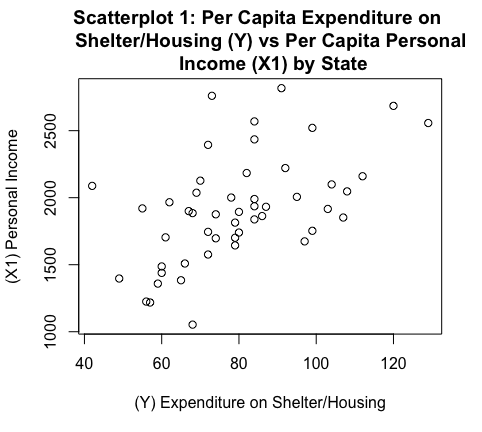
\includegraphics[scale=.80]{Scatterplot1.png}
		Description of Scatterplot 1: It looks like there is a slight positive, linear relationship between Per Capita Income and Expenditure on Housing based on this graph, because as y increases, x tends to increase as well.
		\end{center}
	
		\newpage	
		\lstinputlisting[language=R, firstline=219, lastline=224]{PS01.R} 
	
		\begin{center}
		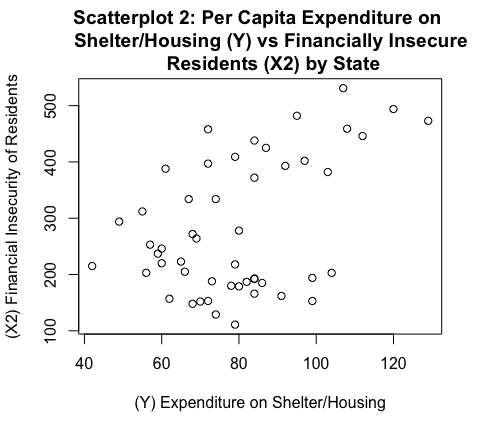
\includegraphics[scale=.80]{Scatterplot2.png}
		Description of Scatterplot 2: It looks like there is less correlation between Financial security of residents and expenditure on shelter/housing based on this graph (especially if compared to the relationship observed in Scatterplot 1), but there could still be a weak positive correlation between the two variables.
		\end{center}
	
		\newpage	
		\lstinputlisting[language=R, firstline=231, lastline=236]{PS01.R} 
		
		\begin{center}
		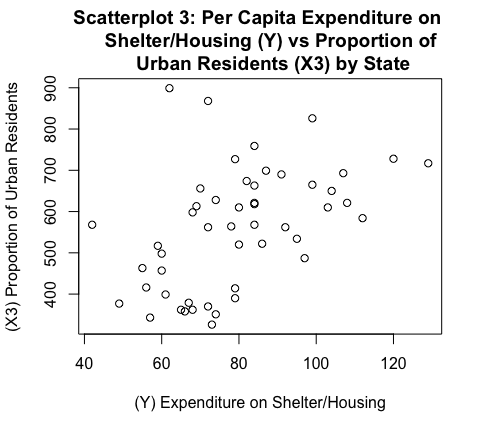
\includegraphics[scale=.80]{Scatterplot3.png}
		Description of Scatterplot 3: It looks like there is a positive, relatively linear relationship between the proportion of urban residents and Expenditure on Housing in a state based on this graph, because as y increases, x tends to increase as well. 
		\end{center}
	
		\newpage	
		\lstinputlisting[language=R, firstline=242, lastline=247]{PS01.R} 
		
		\begin{center}
		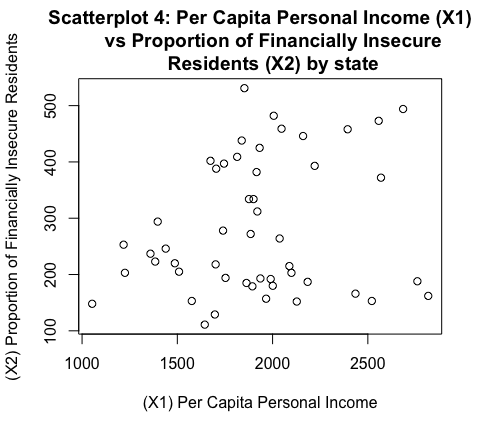
\includegraphics[scale=.80]{Scatterplot4.png}
		Description of Scatterplot 4: It looks like there is no correlation (or at the very least, a very weak positive relationship) between Per Capita Income and Financially Insecure Residents in a state based on this graph.
		\end{center}
	
		\newpage	
		\lstinputlisting[language=R, firstline=253, lastline=258]{PS01.R} 
		
		\begin{center}
		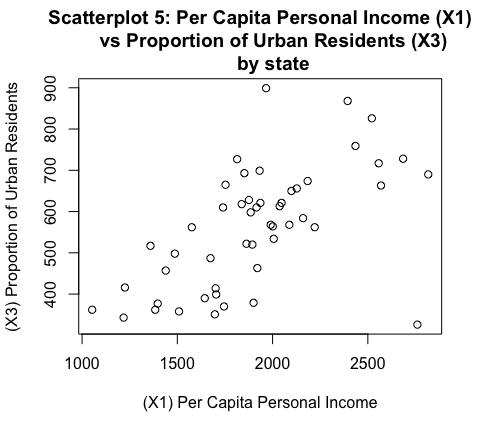
\includegraphics[scale=.80]{Scatterplot5.png}
		Description of Scatterplot 5: It looks like there is a strong (compared to the other graphs) positive, linear relationship between Per Capita Income and proportion of urban residents in a state based on this graph, because as y increases, x tends to increase as well, and these points are closer to one another in a linear shape, with less outliers (though there are a few potential outliers observable).
		\end{center}
	
		\newpage	
		\lstinputlisting[language=R, firstline=266, lastline=271]{PS01.R} 
		
		\begin{center}
		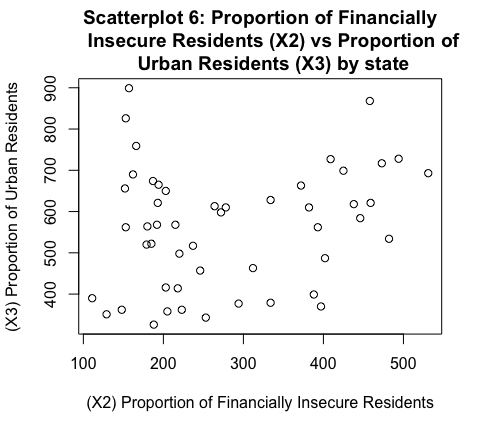
\includegraphics[scale=.80]{Scatterplot6.png}
		Description of  Scatterplot 6: It looks like there is little to no correlation between the proportion of urban residents and proportion of financially insecure residents in a state based on this graph, as there does not seem to be any linear relationship in any direction. In comparison to the other 5 Scatterplots, these two variables seem to have the least / weakest correlation with each other. 
		\end{center}
	
	
		\newpage	
		\item
		Please plot the relationship between \emph{Y} and \emph{Region}? On average, which region has the highest per capita expenditure on housing assistance?
		\vspace{.5cm}
		
		My first step in answering this question is to create the object "Region" in R.  I do this with the following inputs:
		
		\lstinputlisting[language=R, firstline=284, lastline=284]{PS01.R} 
		
		I then create a data.frame object in R that binds the two variables (Region and Y) with the following inputs:
		
		\lstinputlisting[language=R, firstline=288, lastline=288]{PS01.R} 
		
		Now, I create the box plot that shows the variation in State level per-capita expenditure on housing assistance/shelters in each Region (1-4), by inputting the following code into R:
		
		\lstinputlisting[language=R, firstline=293, lastline=298]{PS01.R} 
		
		And this produces Boxplot 1 (on next page):
		\begin{center}
		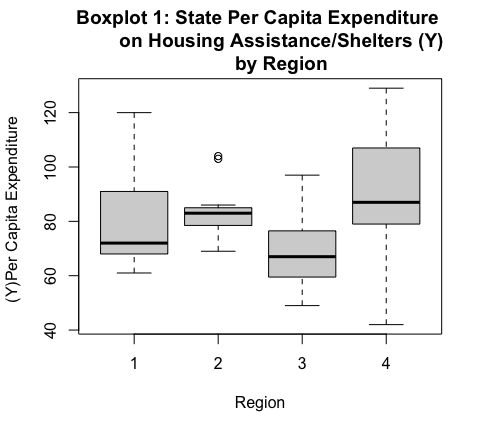
\includegraphics[scale=.80]{Boxplot1.png}
		\end{center}
		
		On average, Region 4 (West) has the highest per capita expenditure on housing assistance.  This is observable in Boxplot 1, as we can see the mean (black line) is close to 90, and higher than the means of all other regions. Because the mean = the average, we can see that the average expenditure on assistance is highest in Region 4 (West).
		
		\newpage
		\item
		Please plot the relationship between \emph{Y} and \emph{X1}? Describe this graph and the relationship. Reproduce the above graph including one more variable \emph{Region} and display different regions with different types of symbols and colors.
		
		This relationship between Y (Expenditure on Housing Assistance/Shelter)and X1 (Per Capita Personal Income) by state was plotted in part 1 of this question.  The scatterplot that was produced (Scatterplot 1) is below:
		
		\begin{center}	
		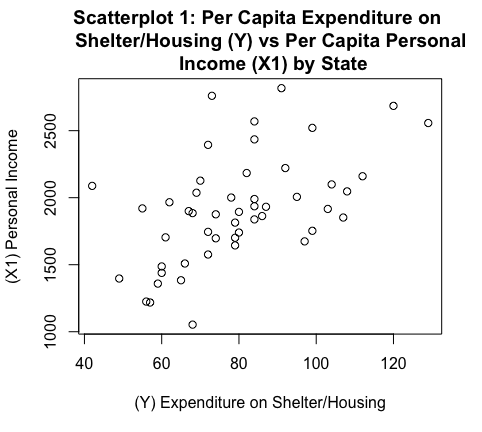
\includegraphics[scale=.80]{Scatterplot1.png}
		\end{center}
		And based on this graph, it seems Y and X1 have a positive, linear relationship. This is because we can see that when Per Capita Income (X1) increases, Expenditure on Housing (Y) also seems to increase on the graph. To understand if there are differences in these values / trends that occur depending on the Region a state is in, we add the Region variable to this plot.
		
		My first step in adding the Variable, Region, is to turn the Region section of the expenditure data into a Factor with 4 levels
		(1, 2, 3, and 4). I do this so that each Region will be a different colour on the graph, rather than each region being a gradation of the same colour. My inputs to turn Region into a Factor with 4 levels is below:
		
		\lstinputlisting[language=R, firstline=326, lastline=326]{PS01.R} 
		
		Then, I produce Scatterplot 7 with this code, which will separate the initial scatterplot (Scatterplot 1) by Region, using 4 different colours to indicate the 4 different regions:
		
		\lstinputlisting[language=R, firstline=331, lastline=333]{PS01.R} 
		
		This code produces Scatterplot 7, as seen below:
		\begin{center}	
		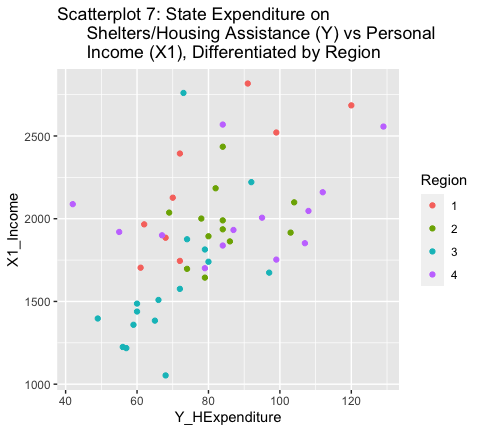
\includegraphics[scale=.80]{Scatterplot7.png}
		\end{center}
		
		
	\end{itemize}
	
	
\end{document}
